% !TEX root = ../utltcp-paper.tex


TCP Hollywood reduces transport latency through support of inconsistent
retransmissions, and by eliminating receiver-side head-of-line blocking. To
quantify the benefits of these two techniques to the application, we begin by
modelling the one-way transport delay, $T_\mathrm{owd}$, as:
\begin{equation}
  T_\mathrm{owd} = T_\mathrm{sender} + T_\mathrm{playout} + T_\mathrm{rtt}/2
  \label{eq:owd}
\end{equation}
where $T_\mathrm{sender}$ is the time taken for the sender to capture,
encode, and transmit a frame of media data. $T_\mathrm{playout}$ is the sum of
the de-jitter buffering delay, and the time taken to decode and render a frame
to the application at the receiver. Finally, $T_\mathrm{rtt}$ is the network
round-trip time. With no loss of generality we assume broadly symmetric network
paths in this analysis.\footnote{This assumption does not hold in ADSL and
cellular networks with asymmetric downstream and upstream links.  In these
cases, our model mis-approximates the application's upper bound on delay,
shifting the line marked ``Application Deadline'' in Figure
\ref{diagram:inconsistentretrans}. While further analysis is needed to
quantify the impact of this, it is clear that it does not change the broad
conclusion of our analysis: that TCP Hollywood increases the usable region of
retransmissions.}

The inter-frame interval of the media, i.e., the duration of media in each frame,
is denoted by $T_\mathrm{framing}$. We know that $T_\mathrm{sender} \geq
T_\mathrm{framing}$, since a frame cannot be sent before it has been captured.
Similarly at the receiver, if the media is to be decoded and rendered without
gaps, then $T_\mathrm{playout} \geq T_\mathrm{framing}$. The time needed to
encode and decode media %can generally be assumed to be
is generally negligible in comparison to the framing interval, making
$T_\mathrm{sender} \approx T_\mathrm{playout}$ a reasonable approximation in the
absence of jitter. At the receiver, however, while the media decoding and
rendering time is generally small, the de-jitter buffer duration can be
significant, and a similar approximation cannot be made.

% For a given application there will be an acceptable delay bound,
The one-way transport delay contributes to an application's acceptable delay
bound
%as set by the application %% slight mod to prevent multi-line inequality.
$T_\mathrm{max}$, such that $T_\mathrm{owd} \leq T_\mathrm{max}$. For
interactive applications, the delay bound is generally around 150ms
\cite{itu:2003:delay}, whereas streaming applications can accept longer delay
bounds (around 0.5 seconds if channel surfing is to be supported; up to tens of
seconds for on-demand streaming).

% We simplify the analysis by assuming that TCP flows
% are steady-state and application-limited. All of these assumptions hold in
% the evaluations described later; our prototype implementation assumes
% symmetric network delay, and the applications we tested generate
% application-limited TCP flows.

%-------------------------------------------------------------------------------
\subsection{Utility of Inconsistent Retransmissions} \label{subsec:rexmit}

TCP senders interpret a triple duplicate acknowledgement as an
indication of packet loss, and retransmit the missing packet. It follows that
the time needed by a sender to identify packet loss following a transmission
has a lower bound of:
\begin{equation}
  \label{eq:retransmission}
  T_\mathrm{rexmit} = T_\mathrm{rtt} + 3 \times T_\mathrm{framing}
\end{equation}

At the receiver there is one additional framing interval to compensate for the
interval that was lost with the original transmission.
% Thus the lower bound for an arrival of a retransmission at the receiver
% $T_\mathrm{rexmit}$ is,
% \begin{equation}
%   \label{eq:retransmission}
%   T_\mathrm{rexmit} = T_\mathrm{rtt} + (3 + 1)\times T_\mathrm{framing} .
% \end{equation}
Assume media decoding and rendering take a negligible time. A
retransmitted packet will arrive in time to be received and rendered to the
application, provided:
\begin{equation}
  \label{eq:playout_lower}
  T_\mathrm{playout} \geq T_\mathrm{rexmit} + T_\mathrm{framing}
\end{equation}
% at its correct time, and it is beneficial to retransmit lost packets.

%However,
When $T_\mathrm{playout} < T_\mathrm{rexmit}$, retransmissions of the
original packet will arrive after the data was scheduled to be rendered, and
will be discarded by the application. This gives a lower bound on
$T_\mathrm{playout}$ for standard TCP retransmission to be useful.

The corresponding upper bound
is the maximum acceptable delay for the application,% $T_\mathrm{owd} =
$T_\mathrm{max}$.
If we assume media encoding delay is negligible, $T_\mathrm{sender} \approx
T_\mathrm{framing}$. By combining these bounds, we see that standard TCP
retransmissions will arrive in time to be rendered to the
application, provided:
\begin{equation}
   T_\mathrm{max} - T_\mathrm{framing} - T_\mathrm{rtt}/2
   \geq
   T_\mathrm{playout} \geq T_\mathrm{rtt} + (3+1) \times T_\mathrm{framing}
\label{eq:standard-rexmit}
\end{equation}

\begin{figure}[t]
\centering
 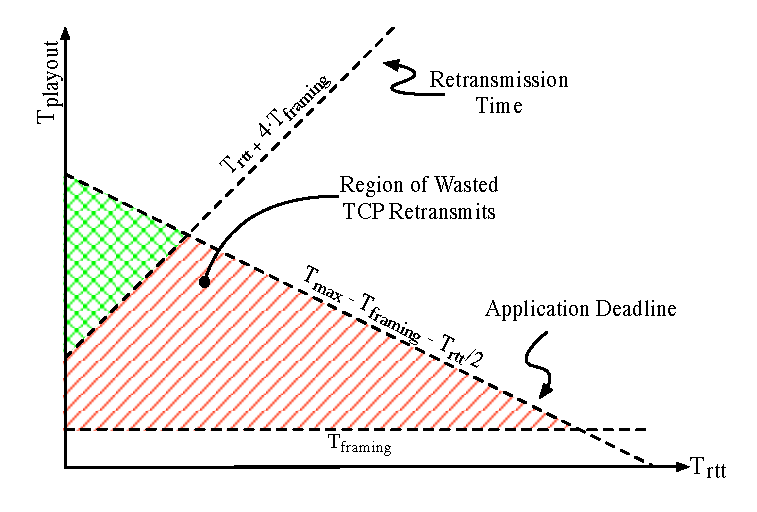
\includegraphics[width=\columnwidth]{figures/analysis-delay-region.pdf}
 \caption{\emph{Inconsistent Retransmissions} for real-time applications: TCP
 retransmissions may arrive too late to be used, if the play-out delay is set
  to meet the application deadline}
\label{diagram:inconsistentretrans}
\end{figure}

This inequality is shown graphically in Figure
\ref{diagram:inconsistentretrans}. The unshaded regions in Figure
\ref{diagram:inconsistentretrans} fall outside of the feasible operating regime
of the application and may be ignored, as they correspond to stalls in play-out
or overall delay bound violations.
% , and may be ignored: and are not part of the feasible operating regime of the
% application.
The feasible operating regime is represented by the shaded regions that separate
useful from wasteful retransmissions. The green cross-hatch highlights the
region where standard TCP retransmissions arrive in time to be useful.

Wasteful TCP retransmissions are marked by the red-lined region in
Figure~\ref{diagram:inconsistentretrans}. When the media play-out delay is less
than the retransmission time ($T_\mathrm{playout} < T_\mathrm{rexmit}$) but
satisfies the overall delay bound ($T_\mathrm{playout} \leq T_\mathrm{max} -
T_\mathrm{framing} - T_\mathrm{rtt}/2$),  and is greater than the framing
interval ($T_\mathrm{playout} \geq T_\mathrm{framing}$), then standard TCP
retransmissions will arrive too late.% to be useful.
% This region is marked with red stripes in
% Figure~\ref{diagram:inconsistentretrans}.
This is where inconsistent retransmissions are useful:
%However, this region can be used with inconsistent retransmissions:
when a TCP retransmission will arrive too late to replace the original lost
packet in this region. By contrast an inconsistent retransmission can use that
retransmission slot to transmit the next unsent data segment. The lost packet is
never recovered, but its sequence number is reused to send useful data.

\begin{table*}[h]
 \centering
 \normalsize
  \input{figures/analysis-utilitycompare.tex}
 \vspace{4mm}
 \caption{Sample TCP and TCP Hollywood RTT bounds required to meet application bounds,
 highlighting indicates where TCP Hollywood is beneficial}
\label{tab:analysis_comparison}
\end{table*}

\subsection{Inconsistent Retransmissions and Real-Time Media}
\label{subsec:realtime}
The benefits of TCP Hollywood can be quantified by substituting real-time
traffic parameters into Equation~\ref{eq:standard-rexmit}.
Consider interactive voice telephony. Widely deployed speech codecs typically
use $T_\mathrm{framing} = 20\mathrm{ms}$ with a delay bound of $T_\mathrm{max} =
150\mathrm{ms}$~\cite{itu:2003:delay}. Assuming media encoding delays are
negligible, so that $T_\mathrm{sender} = T_\mathrm{framing}$, then the feasible
region where standard TCP retransmissions arrive in time to be useful can be
derived from Equation \ref{eq:standard-rexmit} as:
\begin{equation}
  130\mathrm{ms} - T_\mathrm{rtt}/2
  \geq
  T_\mathrm{playout}
  \geq
  T_\mathrm{rtt} + 80\mathrm{ms}
  \label{eq:telephony-delay-bound}
\end{equation}
which has valid solutions for $T_\mathrm{playout}$ provided $T_\mathrm{rtt} \leq
33.33\mathrm{ms}$. This round-trip time bound is low for wide-area networks. For
example, TCP retransmission would be useful for calls from the authors' homes
within Europe, but discarded during inter-continental calls.
%% MF- Eq3 cannot be used to solve inconsistent rexmits where T_playout
%%     must be less than rexmit AND less than deadline but \geq framing.
Figure~\ref{diagram:inconsistentretrans} shows TCP Hollywood
provides valid solutions for $T_\mathrm{playout}$ when $T_\mathrm{rtt} \leq
220\mathrm{ms}$, showing the utility of inconsistent retransmissions for this
application.

For on-demand streaming using MPEG DASH, the framing interval
and delay bounds are typically much larger.  A typical deployment today
might use an encoding segment size of $T_\mathrm{framing} = 2\mathrm{s}$,
and an overall delay bound of $T_\mathrm{max} = 30\mathrm{s}$. Assuming
$T_\mathrm{sender} = T_\mathrm{framing}$, and substituting into Equation
\ref{eq:standard-rexmit}, this permits valid solutions for
$T_\mathrm{playout}$ provided $T_\mathrm{rtt} \leq 13.33\mathrm{s}$,
giving no benefit from inconsistent retransmission.

These two applications represent extremes in
terms of latency bounds: voice telephony has tight latency bounds, while
those of on-demand video streaming are relaxed. We analyse a third
application: IPTV delivery using DASH. IPTV applications seek to minimise
\textit{zap time} (i.e., the total time taken between a viewer selecting
a channel, and content from that channel being displayed). Bouzakaria
et al. \cite{bouzakaria:2014:overhead} show that end-to-end latencies --
the time between encoding and decoding of a frame -- of less than 240ms
can be achieved using DASH. Using their techniques, segments are fragmented
into $200\mathrm{ms}$ chunks for delivery, giving
$T_\mathrm{sender} = T_\mathrm{framing} = 200\mathrm{ms}$. An overall delay
bound of $T_\mathrm{max} = 1\mathrm{s}$ allows for channel surfing to be
supported. Substituting these values into Equation \ref{eq:standard-rexmit},
we see that regular TCP retransmissions do not benefit this application for
any RTT values. In contrast, inconsistent retransmissions in TCP Hollywood can
be used when $T_\mathrm{rtt} \leq 1\mathrm{s}$.

Table \ref{tab:analysis_comparison} summarises the three applications considered.
Utility of inconsistent retransmission is seen to depend on
the latency bounds of the application. Interactive applications, where
the overall latency requirements are tight, can strongly benefit from
the ability to send new data in place of a retransmission, but those
applications with relaxed latency bounds find less benefit.
%-------------------------------------------------------------------------------

\begin{figure*}
\centering
  \subfloat[$T_\mathrm{playout}$ region where blocked segments will be
           delivered too late.]{
           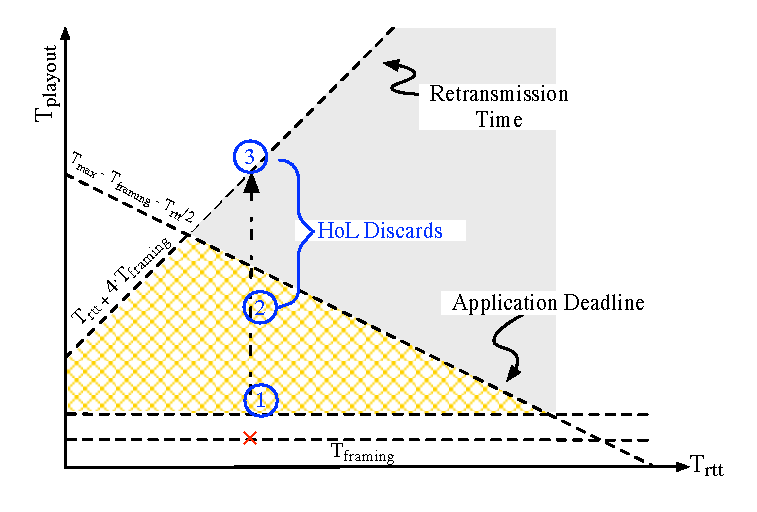
\includegraphics[width=\columnwidth]
           {figures/analysis-HoL-region-v2.pdf}
           \label{subfig:HoLregion}
  } \hfill
  \subfloat[Head of line blocking events between a loss and its
           retransmission.]{
           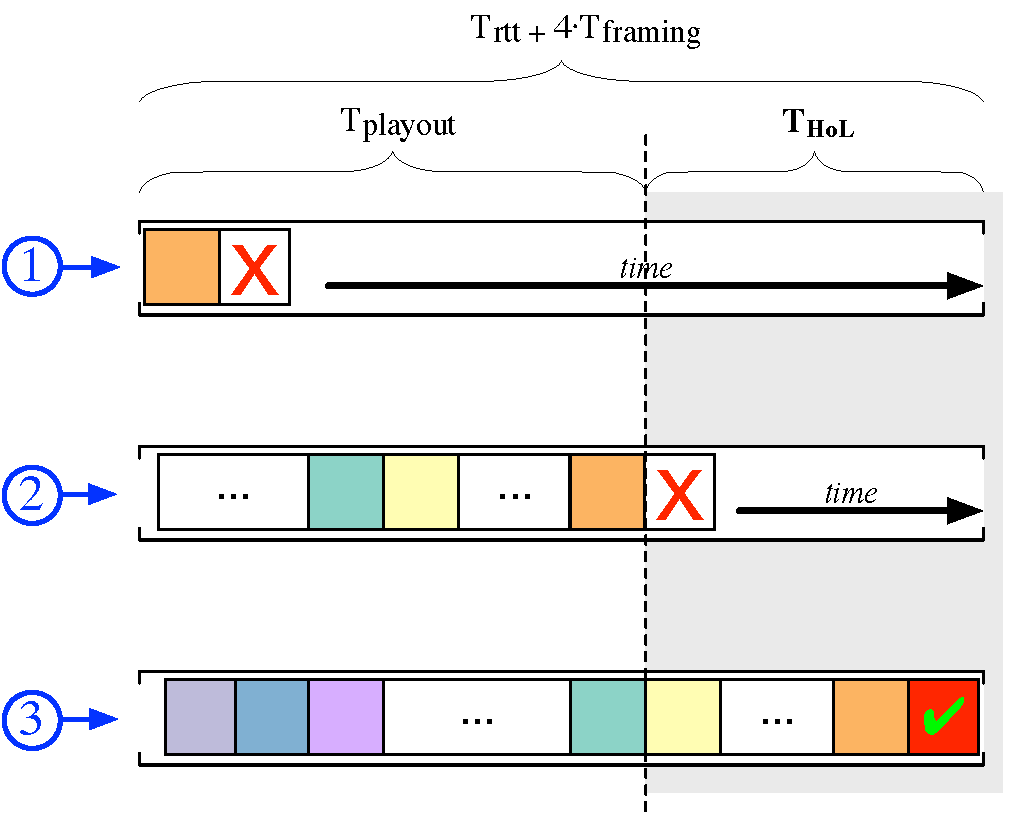
\includegraphics[width=0.9\columnwidth]
           {figures/analysis-HoL-time.pdf}
           \label{subfig:HoLtimed}
  }
 \caption{\emph{Head of line blocking} for real-time applications using regular TCP: for any given
 RTT and playout, segments that immediately follow a loss (1) are pushed
 past the acceptable deadline (2), and delivered as late as (3). The gap between RTT
 and playout is the duration of useful, but HoL blocked segments}
\label{fig:HoLanal}
\end{figure*}


%-------------------------------------------------------------------------------
\subsection{Connecting Head-of-Line Blocking}
\label{subsec:HoL}

If a packet is lost, then TCP will send a retransmission once a triple
duplicate ACK is received. If standard TCP is used, then later segments
will not be delivered to the application until the retransmission of the
lost segment is received, potentially causing media play-out to stall.
This is known as head-of-line blocking, as discussed in Section~\ref{sec:background}.

The size of the play-out buffer relative to the round-trip time and media
framing interval determines whether play-out stalls, or whether there is
sufficient buffering to cover the retransmission delay. From
Equation \ref{eq:playout_lower}, if
$T_\mathrm{playout} \geq T_\mathrm{rexmit} + T_\mathrm{framing}$, then the
retransmission will arrive in time to be played out, and no head-of-line
blocking will occur.

% Otherwise, there will be a period of duration $T_\mathrm{HoL} =
% T_\mathrm{rexmit} + T_\mathrm{framing} - T_\mathrm{playout}$ where the receiver
% is blocked waiting for the retransmission to arrive, and unable to play back
% media.
% %
% Substituting from Equation \ref{eq:retransmission}, this gives
% $T_\mathrm{HoL} = T_\mathrm{rtt} + 4 \times T_\mathrm{framing} -
% T_\mathrm{playout}$. If Equation \ref{eq:standard-rexmit} is satisfied,
% $T_\mathrm{HoL}$ is never positive, and the system cannot suffer from
% head-of-line blocking. If $T_\mathrm{playout}$ is below the minimum bound from
% Equation \ref{eq:standard-rexmit}, then head-of-line blocking can occur.
%
% =============

% TCP implements head-of-line blocking to facilitate in-order delivery. In the
% context of real-time traffic head-of-line blocking imposes additional delay on
% segments that follow a loss.
% Following from the previous discussion, a wasteful segment retransmission in TCP may
% cause some portion of blocked data, that otherwise arrives in time, to also
% become wasteful while waiting for the retransmission. Assuming no losses between
% a loss and its retransmission, then a full $T_\mathrm{rtt}$ of data will be
% delayed by head-of-line blocking. If $T_\mathrm{playout}$ adheres to the lower
% bound \todo{from equation ??} then all delayed segments will be delivered
% on time, despite the head-of-line blocking.

However, if $T_\mathrm{playout} < T_\mathrm{rexmit} + T_\mathrm{framing}$, then
the retransmission will not arrive in time to be played-out. This will cause a
1-segment gap in the media play-out, since some data is missing (this occurs
with both standard TCP, and with the TCP Hollywood extensions). If standard TCP
is used, then the receiver may \emph{also} suffer head-of-line blocking and be
unable to access later segments, leading to a longer gap in play-out.

If the retransmission arrives less than one framing interval after it was
scheduled to be played out, i.e., if
       $T_\mathrm{rexmit} \leq T_\mathrm{playout}
                          < T_\mathrm{rexmit} + T_\mathrm{framing}$
then it will arrive before the following packet is to be played.  In this case,
there is no head-of-line blocking, and only a single packet gap occurs in
play-out. If it is further delayed, such that $T_\mathrm{playout} <
T_\mathrm{rexmit}$, then head-of-line blocking will cause one or more later
frames to also miss their play-out.

A graphical representation is provided by Figure~\ref{fig:HoLanal}. The  yellow
cross-hatch region in Figure~\ref{subfig:HoLregion} is the region of
$T_\mathrm{playout}$ values where blocked segments will be made wasteful. The
details are labeled in Figure~\ref{subfig:HoLregion} by numbered events, with
associated time-lines in Figure~\ref{subfig:HoLtimed}. For a given value of
$T_\mathrm{rtt}$ the process begins with a loss marked by the red
`\textcolor{red}{$\times$}'. The next frame arrives at \textcircled{1} and is held by TCP,
as are all the segments that follow, awaiting the retransmission. For any size
of $T_\mathrm{playout}$ at that moment \textcircled{2}, the retransmission will arrive too
late. Upon arrival of the retransmission \textcircled{3} TCP releases blocked segments to
the play-out buffer. The duration of the head-of-line blocking that will be
discarded by the play-out buffer is labelled as $T_\mathrm{HoL}$ in
Figure~\ref{fig:HoLanal}, can be calculated as:
\begin{equation}
  T_\mathrm{HoL} = T_\mathrm{rexmit} - T_\mathrm{playout}
                 = T_\mathrm{rtt} + 3 \times T_\mathrm{framing} -
                 T_\mathrm{playout}
\label{eq:t-hol}
\end{equation}

The duration translates to $N_\mathrm{HoL}$ frames missing their play-out due to
head of line blocking, and in addition to the retransmission that arrived too
late, where:
\begin{equation}
  N_\mathrm{HoL} =
    \max\left(
      \left\lceil
      \frac{T_\mathrm{rtt} + 3 \times T_\mathrm{framing} - T_\mathrm{playout}}{T_\mathrm{framing}}
      \right\rceil, 0
    \right)
\label{eq:n-hol}
\end{equation}

% A graphical representation is provided by Figure~\ref{fig:HoLanal}.
% The  yellow cross-hatch region in Figure~\ref{subfig:HoLregion} is the region of
% $T_\mathrm{playout}$ values where blocked segments will be made wasteful.
%
% The details are labeled in Figure~\ref{subfig:HoLregion} by numbered events,
% with associated  time-lines in Figure~\ref{subfig:HoLtimed}. For a given value
% of $T_\mathrm{rtt}$ the process begins with a loss marked by the red
% '\textcolor{red}{$\times$}'. The next segment to arrive (1) is held by TCP, as
% are all segments that follow. Then for a given value of $T_\mathrm{playout}$ the
% retransmission (2) will arrive too late. TCP releases blocked segments upon (3)
% the arrival of the retransmission. The duration of blocked segments that will be
% discarded by the play-out buffer, labeled as $T_\mathrm{HoL}$ in
% Figure~\ref{fig:HoLanal}, can be calculated as
%
% \begin{align}
%   T_\mathrm{HoL} & = T_\mathrm{rexmit} - T_\mathrm{playout}
%                      \nonumber \\
%                  & = T_\mathrm{rtt} + 3 \times T_\mathrm{framing} - T_\mathrm{playout} .
% \label{eq:hol}
% \end{align}

Finally, we remark on the grey shaded region in Figure~\ref{subfig:HoLregion}
that occurs  when that when retransmissions arrive past the acceptable deadline.
From Equation~\ref{eq:standard-rexmit}, values of $T_\mathrm{playout}$ are
upper-bound by the application deadline. Subsituting this into
Equation~\ref{eq:t-hol} gives a lower bound on $T_\mathrm{HoL}$ of:
\begin{equation}
  T_\mathrm{HoL} \geq 3 \times T_\mathrm{rtt}/2 + 4 \times T_\mathrm{framing} - T_\mathrm{max}
\label{eq:hol-lower}
\end{equation}
%\begin{align}
%  T_\mathrm{HoL} & \geq T_\mathrm{rtt} + 4 \times T_\mathrm{framing}
%                        - T_\mathrm{max} - T_\mathrm{framing}
%                        - T_\mathrm{rtt}/2 \nonumber \\
%                 & \geq T_\mathrm{rtt}/2 + 3 \times T_\mathrm{framing}
%                        - T_\mathrm{max} .
%\label{eq:hol-lower}
%\end{align}
As $T_\mathrm{rtt}$ increases under TCP, so too does $T_\mathrm{HoL}$, and with
it the fragility of the real-time connection. While a TCP retransmission under
these circumstances will always arrive too late, the TCP Hollywood extensions eliminate
$T_\mathrm{HoL}$. In doing so the grey shaded region in
Figure~\ref{subfig:HoLregion}, where real-time connections may be infeasible
under TCP, are made viable with TCP Hollywood.

Our analysis identifies the value of inconsistent retransmissions, and the
way in which they interact with head-of-line blocking. Specifically, it
shows that removal of head-of-line blocking, via receiver side
modifications to the kernel TCP stack, is necessary to make effective use
of inconsistent retransmissions.  For this reason, a full deployment of
TCP Hollywood eliminates head-of-line blocking, to support latency
reduction and improve good-put due to inconsistent retransmissions.
